\section{eo\-Linear\-Fit\-Scaling$<$ EOT $>$ Class Template Reference}
\label{classeo_linear_fit_scaling}\index{eoLinearFitScaling@{eoLinearFitScaling}}
An instance of {\bf eo\-Perf2Worth}{\rm (p.\,\pageref{classeo_perf2_worth})} COmputes the linearly scaled fitnesses with given selective pressure Pselect(Best) == pressure/size\-Pop Pselect(average) == 1.0/size\-Pop truncate negative values to 0 -.  


{\tt \#include $<$eo\-Linear\-Fit\-Scaling.h$>$}

Inheritance diagram for eo\-Linear\-Fit\-Scaling$<$ EOT $>$::\begin{figure}[H]
\begin{center}
\leavevmode
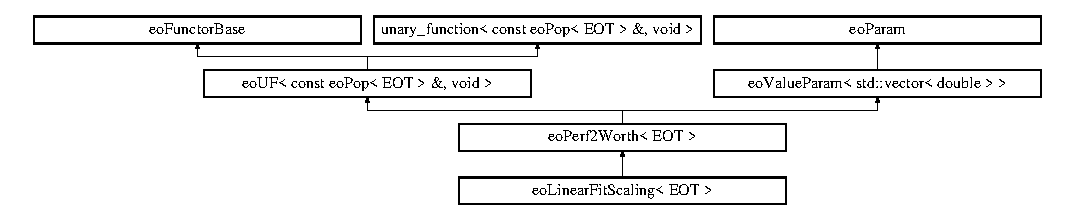
\includegraphics[height=2.52252cm]{classeo_linear_fit_scaling}
\end{center}
\end{figure}
\subsection*{Public Member Functions}
\begin{CompactItemize}
\item 
{\bf eo\-Linear\-Fit\-Scaling} (double \_\-p=2.0)\label{classeo_linear_fit_scaling_a0}

\item 
virtual void {\bf operator()} (const {\bf eo\-Pop}$<$ {\bf EOT} $>$ \&\_\-pop)\label{classeo_linear_fit_scaling_a1}

\begin{CompactList}\small\item\em The pure virtual function that needs to be implemented by the subclass. \item\end{CompactList}\end{CompactItemize}
\subsection*{Private Attributes}
\begin{CompactItemize}
\item 
double {\bf pressure}\label{classeo_linear_fit_scaling_r0}

\end{CompactItemize}


\subsection{Detailed Description}
\subsubsection*{template$<$class EOT$>$ class eo\-Linear\-Fit\-Scaling$<$ EOT $>$}

An instance of {\bf eo\-Perf2Worth}{\rm (p.\,\pageref{classeo_perf2_worth})} COmputes the linearly scaled fitnesses with given selective pressure Pselect(Best) == pressure/size\-Pop Pselect(average) == 1.0/size\-Pop truncate negative values to 0 -. 

to be used within an {\bf eo\-Select\-From\-Worth}{\rm (p.\,\pageref{classeo_select_from_worth})} object 



Definition at line 43 of file eo\-Linear\-Fit\-Scaling.h.

The documentation for this class was generated from the following file:\begin{CompactItemize}
\item 
eo\-Linear\-Fit\-Scaling.h\end{CompactItemize}
